In this subsection the evaluation of the model trained on full nuclei dataset with full set of augmentations is presented. Distributions of number of nuclei and their area are very similar in shape, the corresponding scatter plots form almost linear dependance. Distributions of intensities are less similar, the higher intensity of predicted images is proved here. However, high scores in Pearson and Spearman correlation coefficients (see Table \ref{table:nuclei-downstream-metrics-coefficients}) suggest that distributions are indeed close to each other. The difference between predictions and ground truth might be caused by an absolute value shift, that can be easily fixed.
\begin{figure}[htb]
	\begin{center}
		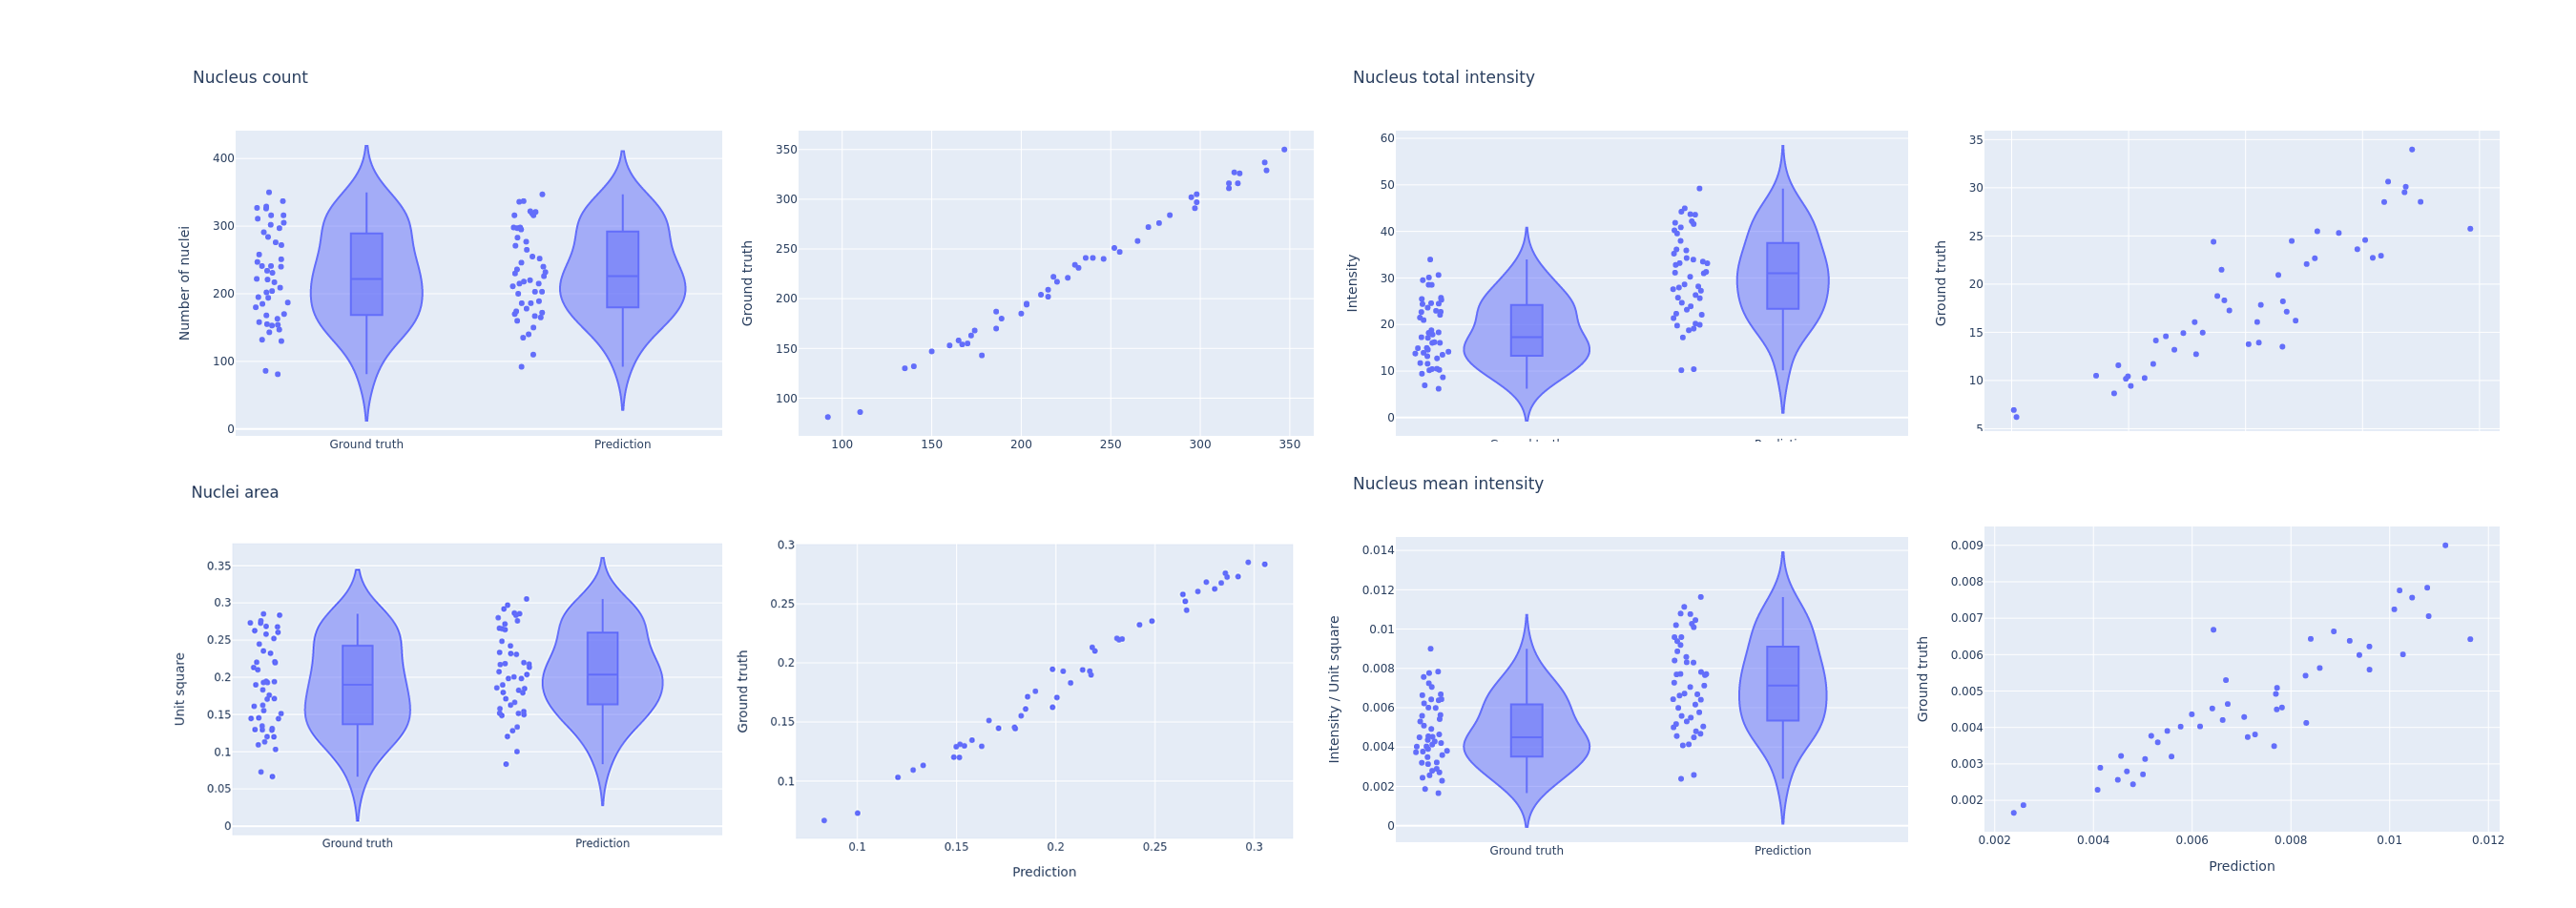
\includegraphics[width=\linewidth]{bilder/nuclei/metric/combined-metrics.png}
		\caption{Metrics for downstream tasks on nuclei}\label{fig:nuclei-downstream-metrics}
	\end{center}
\end{figure}

\begin{table}[htb]
    \centering
    \caption{Correlation coefficients for downstream tasks on nuclei}
        \begin{adjustbox}{width=0.4\textwidth}
            \begin{tabular}{|c|c|c|}\hline
                &Pearson&Spearman
                \\\hline\hline
                Number of nuclei&0.982&0.984\\\hline
                Total intensity&0.867&0.859\\\hline
                Mean intensity&0.882&0.874\\\hline
                Area&0.971&0.976\\\hline
            \end{tabular}
        \label{table:nuclei-downstream-metrics-coefficients}
        \end{adjustbox}
\end{table}
